\documentclass{standalone}
\usepackage{tikz}
\usetikzlibrary{patterns, positioning}
\usetikzlibrary{shapes.misc}
\usepackage[outline]{contour}
\contourlength{1.5pt} 
\usepackage[sfdefault]{ClearSans} %% option 'sfdefault' activates Clear Sans as the default text font
\usepackage[T1]{fontenc}

\begin{document}
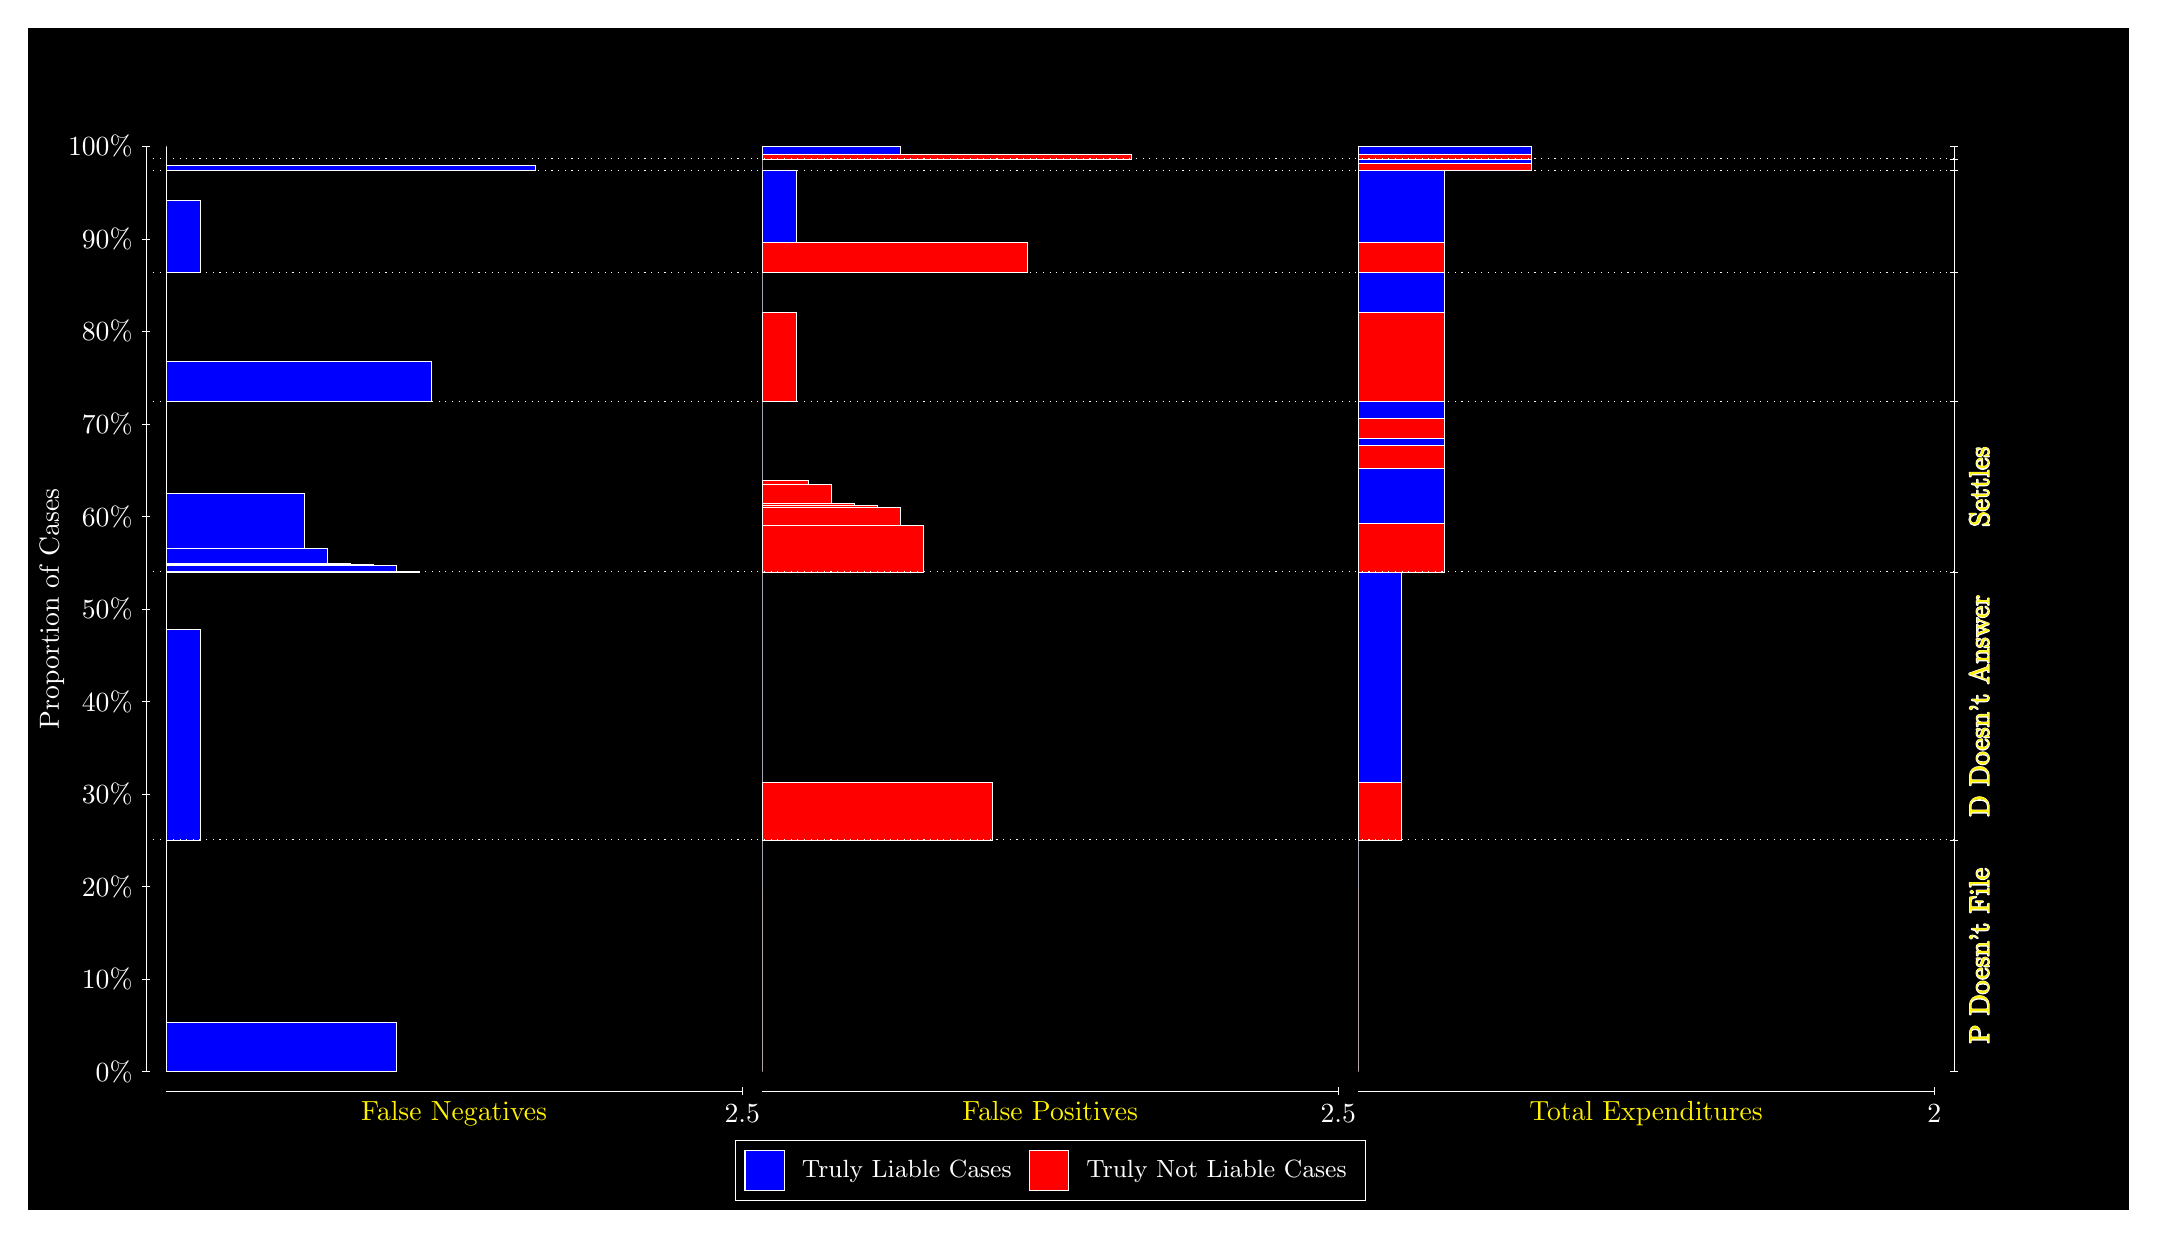
\begin{tikzpicture}
\draw[fill=black] (0,0) rectangle (26.667,15);
\draw[white, very thin] (1.5,1.75) -- (1.5,13.5);
\node[rotate=90, text=white, anchor=center] at (0.3, 7.625) {Proportion of Cases};
\draw[white, very thin] (1.45,1.75) -- (1.55,1.75);
\node[text=white, anchor=east] at (1.45, 1.75) {0\%};
\draw[white, very thin] (1.45,2.925) -- (1.55,2.925);
\node[text=white, anchor=east] at (1.45, 2.925) {10\%};
\draw[white, very thin] (1.45,4.1) -- (1.55,4.1);
\node[text=white, anchor=east] at (1.45, 4.1) {20\%};
\draw[white, very thin] (1.45,5.275) -- (1.55,5.275);
\node[text=white, anchor=east] at (1.45, 5.275) {30\%};
\draw[white, very thin] (1.45,6.45) -- (1.55,6.45);
\node[text=white, anchor=east] at (1.45, 6.45) {40\%};
\draw[white, very thin] (1.45,7.625) -- (1.55,7.625);
\node[text=white, anchor=east] at (1.45, 7.625) {50\%};
\draw[white, very thin] (1.45,8.8) -- (1.55,8.8);
\node[text=white, anchor=east] at (1.45, 8.8) {60\%};
\draw[white, very thin] (1.45,9.975) -- (1.55,9.975);
\node[text=white, anchor=east] at (1.45, 9.975) {70\%};
\draw[white, very thin] (1.45,11.15) -- (1.55,11.15);
\node[text=white, anchor=east] at (1.45, 11.15) {80\%};
\draw[white, very thin] (1.45,12.325) -- (1.55,12.325);
\node[text=white, anchor=east] at (1.45, 12.325) {90\%};
\draw[white, very thin] (1.45,13.5) -- (1.55,13.5);
\node[text=white, anchor=east] at (1.45, 13.5) {100\%};

\draw[white, very thin] (24.457,1.75) -- (24.457,13.5);
\draw[white, very thin] (24.407,1.75) -- (24.507,1.75);
\node[anchor=west] at (24.407, 1.75) {};
\draw[white, very thin] (24.407,4.6929) -- (24.507,4.6929);
\node[anchor=west] at (24.407, 4.6929) {};
\draw[white, very thin] (24.407,8.0956) -- (24.507,8.0956);
\node[anchor=west] at (24.407, 8.0956) {};
\draw[white, very thin] (24.407,10.259) -- (24.507,10.259);
\node[anchor=west] at (24.407, 10.259) {};
\draw[white, very thin] (24.407,11.902) -- (24.507,11.902);
\node[anchor=west] at (24.407, 11.902) {};
\draw[white, very thin] (24.407,13.195) -- (24.507,13.195);
\node[anchor=west] at (24.407, 13.195) {};
\draw[white, very thin] (24.407,13.341) -- (24.507,13.341);
\node[anchor=west] at (24.407, 13.341) {};
\draw[white, very thin] (24.407,13.5) -- (24.507,13.5);
\node[anchor=west] at (24.407, 13.5) {};

\draw[white, very thin, fill=blue] (1.75,1.75) rectangle (4.6775,2.3735);
\draw[white, very thin, fill=red] (1.75,2.3735) rectangle (1.75,4.6929);
\draw[white, very thin, fill=blue] (1.75,4.6929) rectangle (2.1891,7.3661);
\draw[white, very thin, fill=red] (1.75,7.3661) rectangle (1.75,8.0956);
\draw[white, very thin, fill=blue] (1.75,8.0956) rectangle (4.9703,8.1088);
\draw[white, very thin, fill=blue] (1.75,8.1088) rectangle (4.6775,8.1759);
\draw[white, very thin, fill=blue] (1.75,8.1759) rectangle (4.3848,8.1863);
\draw[white, very thin, fill=blue] (1.75,8.1863) rectangle (4.092,8.2099);
\draw[white, very thin, fill=blue] (1.75,8.2099) rectangle (3.7993,8.3998);
\draw[white, very thin, fill=blue] (1.75,8.3998) rectangle (3.5065,9.0915);
\draw[white, very thin, fill=red] (1.75,9.0915) rectangle (1.75,10.259);
\draw[white, very thin, fill=blue] (1.75,10.259) rectangle (5.1167,10.774);
\draw[white, very thin, fill=red] (1.75,10.774) rectangle (1.75,11.902);
\draw[white, very thin, fill=blue] (1.75,11.902) rectangle (2.1891,12.812);
\draw[white, very thin, fill=red] (1.75,12.812) rectangle (1.75,13.195);
\draw[white, very thin, fill=blue] (1.75,13.195) rectangle (6.4341,13.256);
\draw[white, very thin, fill=red] (1.75,13.256) rectangle (1.75,13.341);
\draw[white, very thin, fill=red] (1.75,13.341) rectangle (1.75,13.404);
\draw[white, very thin, fill=blue] (1.75,13.404) rectangle (1.75,13.5);
\draw[white, very thin, fill=red] (9.3189,1.75) rectangle (9.3189,4.0693);
\draw[white, very thin, fill=blue] (9.3189,4.0693) rectangle (9.3189,4.6929);
\draw[white, very thin, fill=red] (9.3189,4.6929) rectangle (12.246,5.4225);
\draw[white, very thin, fill=blue] (9.3189,5.4225) rectangle (9.3189,8.0956);
\draw[white, very thin, fill=red] (9.3189,8.0956) rectangle (11.368,8.6896);
\draw[white, very thin, fill=red] (9.3189,8.6896) rectangle (11.075,8.9147);
\draw[white, very thin, fill=red] (9.3189,8.9147) rectangle (10.783,8.9467);
\draw[white, very thin, fill=red] (9.3189,8.9467) rectangle (10.49,8.9676);
\draw[white, very thin, fill=red] (9.3189,8.9676) rectangle (10.197,9.2102);
\draw[white, very thin, fill=red] (9.3189,9.2102) rectangle (9.9044,9.263);
\draw[white, very thin, fill=blue] (9.3189,9.263) rectangle (9.3189,10.259);
\draw[white, very thin, fill=red] (9.3189,10.259) rectangle (9.758,11.387);
\draw[white, very thin, fill=blue] (9.3189,11.387) rectangle (9.3189,11.902);
\draw[white, very thin, fill=red] (9.3189,11.902) rectangle (12.686,12.286);
\draw[white, very thin, fill=blue] (9.3189,12.286) rectangle (9.758,13.195);
\draw[white, very thin, fill=red] (9.3189,13.195) rectangle (9.3189,13.279);
\draw[white, very thin, fill=blue] (9.3189,13.279) rectangle (9.3189,13.341);
\draw[white, very thin, fill=red] (9.3189,13.341) rectangle (14.003,13.404);
\draw[white, very thin, fill=blue] (9.3189,13.404) rectangle (11.075,13.5);
\draw[white, very thin, fill=red] (16.888,1.75) rectangle (16.888,4.0693);
\draw[white, very thin, fill=blue] (16.888,4.0693) rectangle (16.888,4.6929);
\draw[white, very thin, fill=red] (16.888,4.6929) rectangle (17.437,5.4225);
\draw[white, very thin, fill=blue] (16.888,5.4225) rectangle (17.437,8.0956);
\draw[white, very thin, fill=red] (16.888,8.0956) rectangle (17.986,8.7105);
\draw[white, very thin, fill=blue] (16.888,8.7105) rectangle (17.986,9.4126);
\draw[white, very thin, fill=red] (16.888,9.4126) rectangle (17.986,9.708);
\draw[white, very thin, fill=blue] (16.888,9.708) rectangle (17.986,9.7882);
\draw[white, very thin, fill=red] (16.888,9.7882) rectangle (17.986,10.045);
\draw[white, very thin, fill=blue] (16.888,10.045) rectangle (17.986,10.259);
\draw[white, very thin, fill=red] (16.888,10.259) rectangle (17.986,11.387);
\draw[white, very thin, fill=blue] (16.888,11.387) rectangle (17.986,11.902);
\draw[white, very thin, fill=red] (16.888,11.902) rectangle (17.986,12.286);
\draw[white, very thin, fill=blue] (16.888,12.286) rectangle (17.986,13.195);
\draw[white, very thin, fill=red] (16.888,13.195) rectangle (19.083,13.279);
\draw[white, very thin, fill=blue] (16.888,13.279) rectangle (19.083,13.341);
\draw[white, very thin, fill=red] (16.888,13.341) rectangle (19.083,13.404);
\draw[white, very thin, fill=blue] (16.888,13.404) rectangle (19.083,13.5);
\draw[white, dotted] (1.5,4.6929) -- (24.457,4.6929);
\draw[white, dotted] (1.5,8.0956) -- (24.457,8.0956);
\draw[white, dotted] (1.5,10.259) -- (24.457,10.259);
\draw[white, dotted] (1.5,11.902) -- (24.457,11.902);
\draw[white, dotted] (1.5,13.195) -- (24.457,13.195);
\draw[white, dotted] (1.5,13.341) -- (24.457,13.341);
\draw[white, very thin] (1.75,1.5) -- (9.0689,1.5);
\node[text=yellow, anchor=north] at (5.4094, 1.5) {False Negatives};
\draw[white, very thin] (9.0689,1.45) -- (9.0689,1.55);
\node[text=white, anchor=north] at (9.0689, 1.45) {2.5};

\draw[white, very thin] (9.3189,1.5) -- (16.638,1.5);
\node[text=yellow, anchor=north] at (12.978, 1.5) {False Positives};
\draw[white, very thin] (16.638,1.45) -- (16.638,1.55);
\node[text=white, anchor=north] at (16.638, 1.45) {2.5};

\draw[white, very thin] (16.888,1.5) -- (24.207,1.5);
\node[text=yellow, anchor=north] at (20.547, 1.5) {Total Expenditures};
\draw[white, very thin] (24.207,1.45) -- (24.207,1.55);
\node[text=white, anchor=north] at (24.207, 1.45) {2};

\node[text=yellow, centered, rotate=90] at (24.777, 3.2214) {\contour{white}{P Doesn't File}};
\node[text=yellow, centered, rotate=90] at (24.777, 6.3943) {\contour{white}{D Doesn't Answer}};
\node[text=yellow, centered, rotate=90] at (24.777, 9.1772) {\contour{white}{Settles}};





\draw (12.978300999999998,1.5) node[draw=none] (baseCoordinate) {};
\begin{scope}[align=center]
        \matrix[scale=0.5, draw=white, below=0.5cm of baseCoordinate, nodes={draw}, column sep=0.1cm]{
            \node[rectangle, draw, minimum width=0.5cm, minimum height=0.5cm, fill=blue] {}; &
            \node[draw=none, font=\small, text=white] (B) {Truly Liable Cases}; &
            \node[rectangle, draw, minimum width=0.5cm, minimum height=0.5cm, fill=red] {}; &
            \node[draw=none, font=\small, text=white] (B) {Truly Not Liable Cases}; \\
            };
\end{scope}

\end{tikzpicture}
\end{document}